\documentclass{article}
\usepackage{amsmath}
\usepackage{amssymb}
\usepackage{setspace}
\usepackage{tasks}
\usepackage{graphicx}
\usepackage{float}
\usepackage{listings}
\newcommand{\norm}[1]{\lVert#1\rVert}
\renewcommand{\vec}[1]{\textbf{#1}}
\begin{document}
\onehalfspacing
\begin{center}
	\section*{\textbf{Class 11}}
	\subsection*{Chapter 10 - STRAIGHT LINES}
\end{center}
The following problem is question 11 from exercise 10.4
\begin{enumerate}
    \item Find the equation of the lines through the point (3, 2) which make an angle of 45\textdegree \hspace{0.1cm} with the line x – 2y = 3.
\end{enumerate}
\textbf{Solution:}\\
The given line can be written as 
\begin{align}
    y=\frac{1}{2}x-\frac{3}{2}
\end{align}
which is of the form
\begin{align}
    y=mx+c
\end{align}
Thus,slope of the given line \begin{align}
    m_2=\frac{1}{2}
\end{align}
It is given that the angle between the required line and line x-2y=3 is 45\textdegree.we know that if $\theta$ is acute angle between lines $l_1$ and $l_2$ with slopes $m_1$ and $m_2$ respectively,then
\begin{align}
tan\theta=\frac{|{m_1-m_2}|}{1+m_1m_2}\\
\implies tan45^\circ=\frac{|{m_1-m_2}|}{1+m_1m_2}\\
\implies 1=\left | \frac{\frac{1}{2}-m_1}{1+\frac{m_1}{2}} \right|\\
\implies 1=\left |\frac{\frac{1-2m_1}{2}}{\frac{2+m_1}{2}} \right|\\
\implies 1=\left|\frac{1-2m_1}{2+m_1}\right|\\
\implies 1=\pm \left(\frac{1-2m_1}{2+m_1}\right)\\
\implies 1=\left(\frac{1-2m_1}{2+m_1}\right)\hspace{0.3cm} and\hspace{0.3cm}  1=- \left(\frac{1-2m_1}{2+m_1}\right)
\end{align}
\begin{align}
    2+m_1=1-2m_1 \hspace{0.3cm} or \hspace{0.3cm} 2+m_1=-1+2m_1\\
    \implies m_1=-\frac{1}{3} \hspace{0.3cm}or\hspace{0.3cm}m_1=3
\end{align}
Now,when $m_1$=3 then,\\
The equation of line passing through (3,2) and having a slope of 3 is:
\begin{align}
    y-2=3(x-3)\\
    \implies y-2=3x-9\\
    3x-y=7
\end{align}
And, when $m_1=-\frac{1}{3}$
The equation of the line passing through (3,2) and having a slope of$ -\frac{1}{3}$is:
\begin{align}
    y-2=-\frac{1}{3}(x-3)\\
    3y-6=-x+3\\
    x+3y=9
\end{align}
Therefore,the equations of the lines are 
\begin{align}
    3x-y=7 \hspace{0.3cm}and\hspace{0.3cm} x+3y=9.
\end{align}
\begin{figure}[H]
\centering
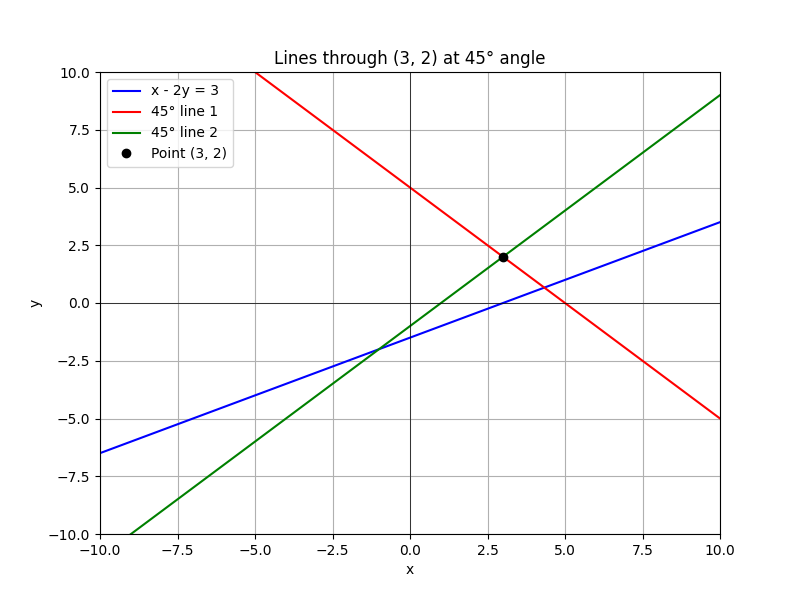
\includegraphics[width=0.7\textwidth]{figs/line.jpg}
\caption{STRAIGHT LINES}
\label{fig:line.jpg}
\end{figure}




\end{document}
